\chap{Résumé des blocs VPL}\label{a.blocks}

\sect{Blocs événement}

\blksm{event-buttons} \textbf{Les boutons}.
Cliquez sur un ou plusieurs boutons;
ils deviendront rouge. Un événement sera déclenché chaque fois que les boutons rouges sont touchés.

\bigskip\bigskip

\blksm{event-prox} \textbf{Capteurs horizontaux} (cinq à l'avant du Thymio et deux à l'arrière).
Cliquez sur un ou plusieurs des petits carrés: ils changeront de couleur.
Initiallement, tous les carrés sont gris, ce qui signifie que les mesures de tous les capteurs seront 
ignorées.

Si le carré est blanc avec un bord rouge \blksm{center-prox}, un événement est déclenché
si beaucoup de lumière est réfléchie.

Si le carré est noir \blksm{center-no-prox}, un événement est déclenché si peu de lumière est réfléchie.

\bigskip

\trickbox{Les objets ordinaires doivent être très proches du Thymio pour pouvoir être détectés
par les capteurs horizontaux. Vous pouvez augmenter de beaucoup la portée des capteurs
en collant du \emph{ruban adhésif réflecteur} comme on en utilise sur les vélos sur les objets.
\footnote{Je remercie Francesco Mondada pour m'avoir donné ce truc!}\\
Comparez l'image suivante avec la \cref{fig.cat-mouse}:
\begin{center}
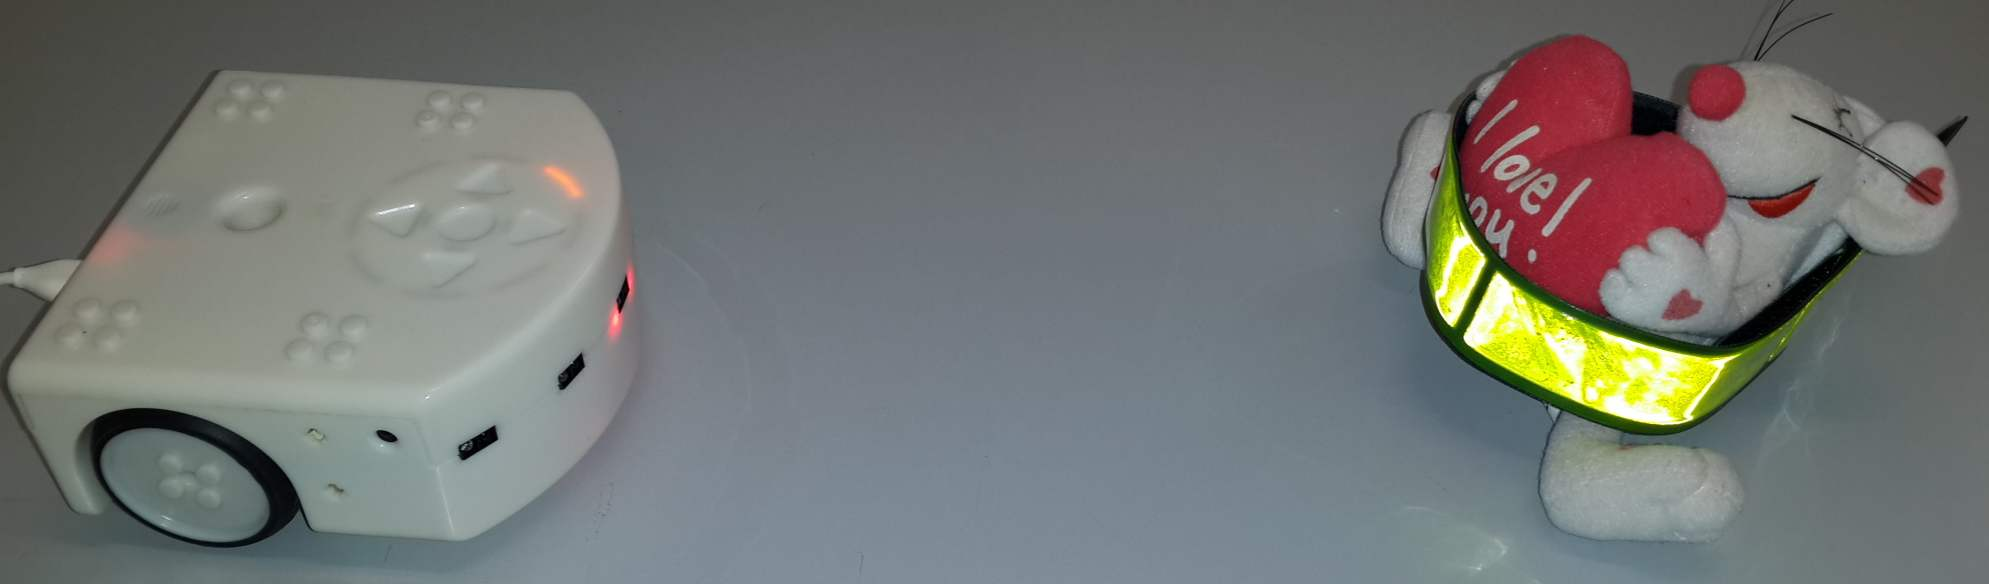
\includegraphics[width=0.8\textwidth]{reflect}
\end{center}
}

\bigskip

\blksm{event-prox-ground} \textbf{Capteurs du sol} (deux sur le dessous du Thymio).
Ce bloc s'utilise de la même façon que les capteurs horizontaux.

\bigskip\bigskip

\blksm{event-prox-advanced}, \blksm{event-prox-ground-advanced} \textbf{Capteurs, mode avancé}.
Ces blocs s'utilisent comme les blocs précédents. Le \emph{slider} du haut change le seuil au-dessus duquel un objet est détecté et le \emph{slider} du bas change le seuil au-dessous duquel l'absence d'un
objet est détectée.

\bigskip\bigskip

Il y a un mode additionnel (le carré est gris foncé \blksm{slow-mid})
dans lequel un événement est déclenché lorsque la valeur mesurée est entre le seuil supérieur et
le seuil inférieur.

\bigskip\bigskip\bigskip

\blksm{event-tap} \textbf{tape}. Un événement est déclenché lorsqu'on donne une petite tape au Thymio.

\bigskip\bigskip\bigskip

\blksm{event-tap-advanced} \textbf{tape, mode avancé}.
Ce bloc s'utilise comme le bloc précédent.
Cliquez sur le petit cercle au centre ou à droite pour passer à l'événement accéléromètre.

\bigskip\bigskip

\blksm{event-roll}, \blksm{event-pitch} \textbf{Accéléromètre, mode avancé}.
Déplacez l'angle blanc dans le demi-cercle vers la droite ou la gauche.
Un événement sera déclenché lorsque l'angle droite/gauche, respectivement avant/arrière 
du Thymio est à l'intérieur de cet intervalle.

\bigskip\bigskip\bigskip\bigskip

\blksm{event-state} \textbf{Événement état, mode avancé}.
L'événement est déclenché seulement si les différents quartiers de l'état actuel
correspondent aux quartiers orange et blancs de ce bloc.
Les quartiers de l'état actuel correspondant aux quartiers gris de ce bloc ne doivent pas forcément
être de la même couleur.

\bigskip

\sect{Blocs action}

\blksm{action-motors} \textbf{Moteurs}.
Déplacez les \emph{sliders} gauche et droite vers le haut pour augmenter la rotation en avant des
moteurs gauche et droit.
Déplacez ces \emph{sliders} vers le bas pour augmenter la rotation en arrière des moteurs
gauche et droit.

\bigskip\bigskip

\blksm{action-colors-up} \textbf{Lumières du haut}.
Déplacez les trois \emph{sliders} vers la droite pour augmenter l'intensité de rouge, de vert,
respectivement de bleu des lumières du haut.

\bigskip\bigskip

\blksm{action-colors-down} \textbf{Lumières du bas}.
Permet d'allumer les lumières du bas. Ce bloc s'utilise comme le bloc précédent.

\bigskip\bigskip\bigskip\bigskip

\blksm{action-music} \textbf{Musique}.
Les six petits cercles représentent des notes de musique.
Une note noire est courte tandis qu'une note blanche est longue.
Cliquez sur un cercle pour changer sa longueur.
Les cinq barres horizontales représentent les différentes hauteurs de notes disponibles.
Cliquez sur une des barres pour placer une note sur cette barre.

\bigskip\bigskip

\blksm{action-timer} \textbf{Minuteur, mode avancé}
Le minuteur peut être reglé pour une durée allant jusqu'à quatre secondes.
Cliquez où vous voulez sur le cercle blanc qui représente le cadran d'un réveil.
Il y aura alors une courte animation et la durée jusqu'à l'alarme sera coloré en bleu.

\bigskip\bigskip

\blksm{action-states} \textbf{États, mode avancé}
Les quatre quartiers du bloc correspondent aux quatre quartiers d'un état.
Cliquez sur un des quartiers pour le mettre en gris, orange ou blanc.

\sect{Remarques concernant les blocs VPL}

\informationbox{Tourner sur place ou doucement}{
Lorsque les moteurs tournent à la même vitesse dans des sens différents, le robot tourne sur place.
Si, au contraire, un seul moteur est allumé, le robot ira à la fois vers l'avant et tournera
vers le côté opposé à celui du moteur allumé. Il vous faudra peut-être mettre plus de puissance 
dans les moteurs pour compenser le frottement du sol.}

\informationbox{Événements capteurs rapidement répétés}{
Dans la plupart des projets, on attribue une couleur (blanc, noir ou gris foncé) à un carré dans 
un bloc capteur pour indiquer que le capteur correspondant joue un rôle
pour déterminer quand les actions associées seront exécutées.
Cepandant, si vous laissez tous les capteurs dans leur couleur grise originale, alors aucune
condition ou restriciton n'est imposée.
L'événement sera alors déclenché 10 fois par secondes, peu importe les valeurs mesurées par les capteurs.}

\informationbox{Événements boutons rapidement répétés}{
La même remarque vaut pour les événements boutons, avec la différence que ceux-ci sont déclenchés
20 fois par seconde.}
